% ============================================================
%  Manuel d'Utilisation -- IoT Controller PWA
%  AOUAS Liza -- Master 1 EEA MTI -- Universite de Lorraine
%  Version amelioree v2.0 -- Juin 2026
% ============================================================
\documentclass[a4paper,12pt]{article}

% --- Encodage ---
\usepackage[T1]{fontenc}
\usepackage[utf8]{inputenc}
\usepackage{times}
\usepackage{microtype}

% --- Mise en page ---
\usepackage[
  top=2.5cm, bottom=2.5cm,
  left=2.5cm, right=2.5cm,
  headheight=20pt
]{geometry}

% --- Couleurs ---
\usepackage[dvipsnames,table]{xcolor}
\definecolor{PrimaryBlue}{HTML}{1A3A5C}
\definecolor{AccentBlue}{HTML}{2E75B6}
\definecolor{LightBlue}{HTML}{D6E4F0}
\definecolor{SuccessGreen}{HTML}{1E7A3C}
\definecolor{LightGreen}{HTML}{D4EFDF}
\definecolor{WarnOrange}{HTML}{B8540A}
\definecolor{LightOrange}{HTML}{FAE5D3}
\definecolor{DangerRed}{HTML}{922B21}
\definecolor{LightRed}{HTML}{FADBD8}
\definecolor{TipPurple}{HTML}{6C3483}
\definecolor{LightPurple}{HTML}{EBD5F5}
\definecolor{CodeBg}{HTML}{F0F3F4}
\definecolor{TableHeader}{HTML}{2E75B6}
\definecolor{TableRowAlt}{HTML}{EBF5FB}
\definecolor{BorderGray}{HTML}{BDC3C7}
\definecolor{TextGray}{HTML}{5D6D7E}
\definecolor{TempBlue}{HTML}{1565C0}
\definecolor{TempGreen}{HTML}{2E7D32}
\definecolor{TempRed}{HTML}{C62828}
\definecolor{PresOrange}{HTML}{E65100}
\definecolor{PresGreen}{HTML}{2E7D32}
\definecolor{PresBlue}{HTML}{1565C0}

% --- Boites ---
\usepackage[most]{tcolorbox}
\tcbuselibrary{breakable,skins,listings}

% --- En-tetes ---
\usepackage{fancyhdr}
\usepackage{lastpage}

% --- Tableaux ---
\usepackage{tabularx}
\usepackage{booktabs}
\usepackage{multirow}
\usepackage{array}
\usepackage{colortbl}

% --- Listes ---
\usepackage{enumitem}

% --- Graphiques ---
\usepackage{graphicx}
\usepackage{amssymb}
\usepackage{tikz}
\usetikzlibrary{shapes.geometric,arrows.meta,positioning,fit,backgrounds,shadows.blur}

% --- Hyperliens ---
\usepackage{hyperref}
\hypersetup{
  colorlinks=true,
  linkcolor=AccentBlue,
  urlcolor=AccentBlue,
  pdftitle={Manuel d'Utilisation -- IoT Controller PWA},
  pdfauthor={AOUAS Liza},
}

% ============================================================
%  BOITES PERSONNALISEES
% ============================================================
\tcbset{
  mybox/.style={
    enhanced, breakable,
    boxrule=0.8pt, arc=4pt,
    left=8pt, right=8pt, top=6pt, bottom=6pt,
    attach boxed title to top left={yshift=-2mm, xshift=8mm},
    boxed title style={arc=3pt, boxrule=0pt},
    fonttitle=\bfseries\small,
    before upper={\setlength{\parskip}{4pt}},
  },
}

\newcommand{\infobox}[2]{%
  \begin{tcolorbox}[mybox,
    colback=LightBlue, colframe=AccentBlue,
    colbacktitle=AccentBlue, coltitle=white,
    title={$\triangleright$\enspace #1}]#2\end{tcolorbox}}

\newcommand{\warnbox}[2]{%
  \begin{tcolorbox}[mybox,
    colback=LightOrange, colframe=WarnOrange,
    colbacktitle=WarnOrange, coltitle=white,
    title={$\triangle$\enspace #1}]#2\end{tcolorbox}}

\newcommand{\successbox}[2]{%
  \begin{tcolorbox}[mybox,
    colback=LightGreen, colframe=SuccessGreen,
    colbacktitle=SuccessGreen, coltitle=white,
    title={$\checkmark$\enspace #1}]#2\end{tcolorbox}}

\newcommand{\dangerbox}[2]{%
  \begin{tcolorbox}[mybox,
    colback=LightRed, colframe=DangerRed,
    colbacktitle=DangerRed, coltitle=white,
    title={$\times$\enspace #1}]#2\end{tcolorbox}}

\newcommand{\tipbox}[2]{%
  \begin{tcolorbox}[mybox,
    colback=LightPurple, colframe=TipPurple,
    colbacktitle=TipPurple, coltitle=white,
    title={$\star$\enspace #1}]#2\end{tcolorbox}}

% Commande inline
\newcommand{\cmd}[1]{\texttt{\colorbox{CodeBg}{\textcolor{PrimaryBlue}{#1}}}}

% Badge couleur
\newcommand{\badge}[2]{%
  \tikz[baseline=(t.base)]\node[
    fill=#1, text=white, rounded corners=3pt,
    font=\ttfamily\scriptsize\bfseries,
    inner xsep=5pt, inner ysep=2pt](t){#2};}

% ============================================================
%  EN-TETE ET PIED DE PAGE
% ============================================================
\pagestyle{fancy}
\fancyhf{}
\fancyhead[L]{\small\color{TextGray}\textbf{Manuel d'Utilisation} --- IoT Controller PWA}
\fancyhead[R]{\small\color{TextGray}AOUAS Liza --- Master 1 EEA MTI}
\fancyfoot[L]{\small\color{TextGray}Universit\'e de Lorraine --- UFR SFA}
\fancyfoot[C]{\small\color{TextGray}2025/2026}
\fancyfoot[R]{\small\color{TextGray}Page \thepage\ / \pageref{LastPage}}
\renewcommand{\headrulewidth}{1pt}
\renewcommand{\footrulewidth}{0.4pt}

% ============================================================
%  TITRES DE SECTIONS
% ============================================================
\usepackage{titlesec}
\newcommand{\sectionline}{{\color{AccentBlue}\titlerule[1.5pt]}}
\titleformat{\section}
  {\color{PrimaryBlue}\Large\bfseries}
  {\colorbox{AccentBlue}{\color{white}\enspace\thesection\enspace}}{10pt}{}
  [\sectionline]
\titleformat{\subsection}
  {\color{AccentBlue}\large\bfseries}
  {\thesubsection}{8pt}{}
\titleformat{\subsubsection}
  {\color{PrimaryBlue}\normalsize\bfseries}
  {\thesubsubsection}{6pt}{}
\titlespacing{\section}{0pt}{18pt}{10pt}
\titlespacing{\subsection}{0pt}{12pt}{6pt}

% ============================================================
\begin{document}

% ========================
%  PAGE DE GARDE
% ========================
\newgeometry{top=0cm,bottom=0cm,left=0cm,right=0cm}
\begin{titlepage}

\begin{tikzpicture}[remember picture, overlay]
  % Bande superieure elargie
  \fill[PrimaryBlue] (current page.north west) rectangle
    ([yshift=-7.2cm] current page.north east);
  \fill[AccentBlue] ([yshift=-7.2cm] current page.north west) rectangle
    ([yshift=-7.55cm] current page.north east);
  % Bande inferieure
  \fill[PrimaryBlue] (current page.south west) rectangle
    ([yshift=2.2cm] current page.south east);
  \fill[AccentBlue] ([yshift=2.2cm] current page.south west) rectangle
    ([yshift=2.5cm] current page.south east);
\end{tikzpicture}
\vspace*{1.4cm}
\begin{center}
  {\color{white}\Large\bfseries UNIVERSIT\'E DE LORRAINE}\\[4pt]
  {\color{white!85!PrimaryBlue}\normalsize Institut Sup\'erieur d'\'Electronique et d'Automatique (ISEA)}\\[2pt]
  {\color{white!85!PrimaryBlue}\normalsize UFR Sciences Fondamentales et Appliqu\'ees (SFA)}\\[2pt]
  {\color{white!85!PrimaryBlue}\normalsize Master 1 EEA --- Mesures et Traitement de l'Information (MTI)}\\[2pt]
  {\color{white!70!PrimaryBlue}\small Ann\'ee Universitaire 2025/2026}
\end{center}

\vspace{2.2cm}
\begin{center}
  {\color{TextGray}\small DOCUMENTATION TECHNIQUE}\\[8pt]
  \begin{tcolorbox}[
    enhanced, colback=white, colframe=AccentBlue,
    boxrule=2pt, arc=6pt,
    width=0.88\textwidth,
    halign=center, valign=center,
    left=16pt, right=16pt, top=14pt, bottom=14pt,
  ]
    {\color{PrimaryBlue}\Huge\bfseries Manuel d'Utilisation}\\[8pt]
    {\color{AccentBlue}\Large\bfseries IoT Controller --- Application PWA}\\[10pt]
    {\color{TextGray}\normalsize
    Guide complet d'utilisation du Dashboard de supervision IoT temps r\'eel\\[4pt]
    Temp\'erature, Pression, Commandes, Graphiques, Statistiques}
  \end{tcolorbox}
\end{center}

\vspace{1.8cm}
\begin{center}
\begin{tcolorbox}[
  enhanced, colback=LightBlue!50, colframe=BorderGray,
  boxrule=0.8pt, arc=4pt, width=0.72\textwidth,
]
\renewcommand{\arraystretch}{1.5}
\begin{tabular}{@{}ll@{}}
  \textbf{\color{PrimaryBlue}Auteure :}        & Liza AOUAS \\
  \textbf{\color{PrimaryBlue}Encadrant :}      & M. Fabrice De Almeida Pereira Monteiro \\
  \textbf{\color{PrimaryBlue}Formation :}      & Master 1 EEA --- MTI \\
  \textbf{\color{PrimaryBlue}\'Etablissement :}& Universit\'e de Lorraine --- Metz \\
  \textbf{\color{PrimaryBlue}Ann\'ee :}        & 2025 -- 2026 \\
  \textbf{\color{PrimaryBlue}Version :}        & v2.0 --- Juin 2026 \\
\end{tabular}
\end{tcolorbox}
\end{center}

\vfill
\begin{center}
  {\color{white}\small Manuel d'Utilisation v2.0 --- Universit\'e de Lorraine --- 2025/2026}
\end{center}
\end{titlepage}
\restoregeometry

% ========================
%  TABLE DES MATIERES
% ========================
\thispagestyle{fancy}
\tableofcontents
\newpage

% ============================================================
\section{Pr\'esentation g\'en\'erale de l'application}
% ============================================================

\textbf{IoT Controller} est une plateforme de supervision industrielle en temps r\'eel
d\'evelopp\'ee dans le cadre du Master 1 MTI \`a l'Universit\'e de Lorraine.
Elle permet de visualiser, analyser et contr\^oler \`a distance les donn\'ees d'un
\'equipement IoT compos\'e d'un microcontr\^oleur ESP8266, d'un capteur environnemental
BMP280 et d'un \'ecran OLED.

L'une des caract\'eristiques majeures de cette application est son \textbf{interface universelle}~:
aucun capteur n'est cod\'e en dur. L'interface se configure automatiquement \`a partir des
m\'etadonn\'ees envoy\'ees par l'\'equipement connect\'e, ce qui la rend adaptable \`a
n'importe quel dispositif IoT sans modification du code.

\vspace{6pt}
\begin{center}
\begin{tcolorbox}[
  enhanced, colback=LightBlue!30, colframe=AccentBlue,
  boxrule=0.8pt, arc=4pt, width=0.92\textwidth,
]
\textbf{\color{PrimaryBlue}Fonctionnalit\'es principales de l'application}

\vspace{6pt}
\begin{itemize}[noitemsep, label=$\checkmark$,
  leftmargin=1.2em, itemsep=2pt]
  \item Affichage temps r\'eel temp\'erature et pression avec code couleur
  \item Graphique Plotly.js interactif --- historique des 50 derni\`eres mesures
  \item Statistiques dynamiques Min\,/\,Moy\,/\,Max calcul\'ees en session
  \item Envoi de commandes vers l'ESP8266 depuis le navigateur
  \item Simulateur OLED virtuel synchronis\'e avec l'\'ecran physique
  \item Console de logs color\'ee avec mode plein \'ecran
  \item Mode hors-ligne avec conservation des derni\`eres donn\'ees
  \item Th\`eme clair et sombre persistant entre les sessions
  \item Installation comme application native (PWA) sur PC et mobile
  \item Multi-clients simultan\'es via broadcast Socket.IO
\end{itemize}
\end{tcolorbox}
\end{center}

\subsection{Organisation de l'interface}

L'interface est structur\'ee en \textbf{trois colonnes compl\'ementaires} con\c{c}ues pour
maximiser la densit\'e d'information sans surcharger l'\'ecran.

\vspace{6pt}
\renewcommand{\arraystretch}{1.4}
\begin{center}
\begin{tabular}{>{\bfseries\color{PrimaryBlue}}m{3.5cm}
                >{\centering}m{2cm}
                m{8.5cm}}
\rowcolor{TableHeader}
\multicolumn{1}{l}{\color{white}\bfseries Zone} &
\color{white}\bfseries Proportion &
\color{white}\bfseries Contenu \\
\rowcolor{white}
Colonne gauche & 0.85fr &
Valeurs IoT temps r\'eel, statistiques Min/Moy/Max, flux disponibles, \'etat syst\`eme \\
\rowcolor{TableRowAlt}
Colonne centre & 2.2fr &
Simulateur OLED virtuel et graphique temps r\'eel (60\,\% de la largeur) \\
\rowcolor{white}
Colonne droite & 0.85fr &
Panneau de commandes et console de logs \\
\rowcolor{TableRowAlt}
En-t\^ete & 100\,\% &
Horloge temps r\'eel, badge LIVE, boutons th\`eme et connexion \\
\rowcolor{white}
Barre de statut & 100\,\% &
Indicateurs syst\`eme, URL backend, boutons Aide et Configurer \\
\end{tabular}
\end{center}

% ============================================================
\section{D\'emarrage et v\'erification de la connexion}
% ============================================================

\subsection{Ouverture de l'application}

Apr\`es avoir suivi la proc\'edure d\'ecrite dans le \textbf{Manuel d'Installation},
double-cliquez sur l'ic\^one \textbf{IoT Controller} sur votre bureau pour lancer l'application.

\infobox{Ordre de d\'emarrage \`a respecter}{
L'application doit \^etre ouverte \textbf{apr\`es} le d\'emarrage du backend. Si le backend
n'est pas lanc\'e, l'interface affichera imm\'ediatement un bandeau rouge (mode hors-ligne).

\begin{enumerate}[noitemsep, label=\arabic*.]
  \item D\'emarrer le backend : \cmd{node server.js}
  \item D\'emarrer le serveur frontend : \cmd{serve -s dist -l 4173}
  \item Ouvrir l'application IoT Controller
\end{enumerate}
}

\subsection{Indicateurs de connexion}

D\`es le d\'emarrage, la barre de statut affiche l'\'etat de chaque composant.
V\'erifiez que tous les indicateurs sont au vert avant de commencer la supervision.

\renewcommand{\arraystretch}{1.4}
\begin{center}
\begin{tabular}{>{\bfseries\color{PrimaryBlue}}m{3.5cm}
                >{\ttfamily\small}m{3cm}
                m{7cm}}
\rowcolor{TableHeader}
\multicolumn{1}{l}{\color{white}\bfseries Indicateur} &
\multicolumn{1}{l}{\color{white}\bfseries \'Etat normal} &
\multicolumn{1}{l}{\color{white}\bfseries Signification} \\
\rowcolor{white}       Backend    & Connect\'e         & Le serveur Node.js r\'epond correctement \\
\rowcolor{TableRowAlt} MQTT       & Actif              & Le broker HiveMQ est joignable \\
\rowcolor{white}       Appareil   & ESP8266\_Liza      & L'\'equipement IoT est connect\'e et publie \\
\rowcolor{TableRowAlt} Badge LIVE & Vert clignotant    & Des donn\'ees sont re\c{c}ues en temps r\'eel \\
\rowcolor{white}       Dernier flux & \`a l'instant    & Une mesure a \'et\'e re\c{c}ue r\'ecemment \\
\end{tabular}
\end{center}

% ============================================================
\section{Lecture et interpr\'etation des donn\'ees}
% ============================================================

\subsection{Affichage des valeurs en temps r\'eel}

Les valeurs de temp\'erature et de pression sont affich\'ees dans la colonne gauche sous
forme de cartes num\'eriques. Elles se rafra\^ichissent automatiquement \textbf{toutes les 5 secondes}.

Chaque valeur est accompagn\'ee d'un \textbf{code couleur dynamique} qui \'evolue en fonction
des seuils de mesure~:

\vspace{6pt}
\begin{center}
\begin{tabular}{>{\bfseries\color{PrimaryBlue}}m{3cm}
                >{\centering\bfseries}m{2.5cm}
                >{\centering}m{2.5cm}
                m{5.5cm}}
\rowcolor{TableHeader}
\multicolumn{1}{l}{\color{white}\bfseries Grandeur} &
\color{white}\bfseries Couleur &
\color{white}\bfseries Condition &
\color{white}\bfseries Interpr\'etation \\
\rowcolor{TempBlue!20} Temp\'erature & \textcolor{TempBlue}{\textbf{Bleu}}   & $< 20$\,\textdegree{}C      & Temp\'erature froide \\
\rowcolor{TempGreen!20}              & \textcolor{TempGreen}{\textbf{Vert}}  & 20 \`a 30\,\textdegree{}C  & Temp\'erature ambiante normale \\
\rowcolor{TempRed!20}                & \textcolor{TempRed}{\textbf{Rouge}}   & $> 30$\,\textdegree{}C      & Temp\'erature \'elev\'ee \\
\rowcolor{PresOrange!15} Pression    & \textcolor{PresOrange}{\textbf{Orange}} & $< 980$\,hPa              & Pression basse (d\'epression) \\
\rowcolor{PresGreen!15}              & \textcolor{PresGreen}{\textbf{Vert}}  & 980 \`a 1020\,hPa         & Pression atmosph\'erique normale \\
\rowcolor{PresBlue!15}               & \textcolor{PresBlue}{\textbf{Bleu}}   & $> 1020$\,hPa             & Haute pression (anticyclone) \\
\end{tabular}
\end{center}

\subsection{Indicateur de fra\^icheur des donn\'ees}

Sous les valeurs num\'eriques, une \textbf{barre horizontale} indique visuellement la fra\^icheur
des derni\`eres donn\'ees re\c{c}ues. Elle se vide progressivement si aucune nouvelle mesure n'arrive.

\vspace{6pt}
\begin{center}
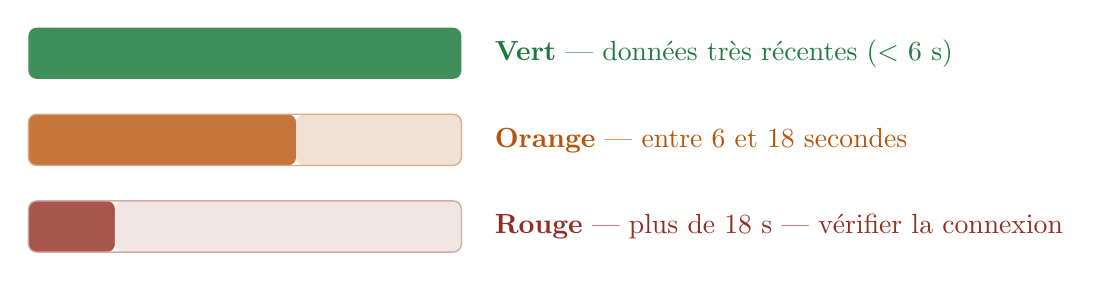
\begin{tikzpicture}[scale=1.0]
  % --- Barre VERTE (pleine) ---
  \fill[SuccessGreen!85, rounded corners=3pt] (0,0) rectangle (5.5, 0.65);
  \node[right] at (5.8, 0.32)
    {\normalsize\color{SuccessGreen}\textbf{Vert} \textemdash{} donn\'ees tr\`es r\'ecentes ($<$ 6 s)};

  % --- Barre ORANGE (mi-pleine) ---
  \fill[WarnOrange!80, rounded corners=3pt] (0,-1.1) rectangle (3.4, -0.45);
  \fill[WarnOrange!18, rounded corners=3pt] (3.4,-1.1) rectangle (5.5, -0.45);
  \draw[WarnOrange!50, rounded corners=3pt, line width=0.5pt] (0,-1.1) rectangle (5.5,-0.45);
  \node[right] at (5.8, -0.78)
    {\normalsize\color{WarnOrange}\textbf{Orange} \textemdash{} entre 6 et 18 secondes};

  % --- Barre ROUGE (presque vide) ---
  \fill[DangerRed!80, rounded corners=3pt] (0,-2.2) rectangle (1.1, -1.55);
  \fill[DangerRed!12, rounded corners=3pt] (1.1,-2.2) rectangle (5.5, -1.55);
  \draw[DangerRed!40, rounded corners=3pt, line width=0.5pt] (0,-2.2) rectangle (5.5,-1.55);
  \node[right] at (5.8, -1.88)
    {\normalsize\color{DangerRed}\textbf{Rouge} \textemdash{} plus de 18 s \textemdash{} v\'erifier la connexion};
\end{tikzpicture}
\end{center}
\vspace{4pt}

\subsection{Statistiques Min/Moy/Max}

Trois badges color\'es affichent les statistiques calcul\'ees \textbf{en temps r\'eel} sur
l'ensemble des mesures de la session en cours.

\begin{center}
\begin{tabular}{>{\centering\bfseries}m{2cm}
                >{\centering}m{3cm}
                m{8cm}}
\rowcolor{TableHeader}
\color{white}Badge &
\color{white}Couleur de fond &
\color{white}Valeur affich\'ee \\
\rowcolor{TempBlue!15}  MIN & Bleu clair  & Valeur minimale depuis le d\'emarrage de la session \\
\rowcolor{TempGreen!15} MOY & Vert clair  & Moyenne arithm\'etique de toutes les mesures \\
\rowcolor{TempRed!15}   MAX & Rouge clair & Valeur maximale depuis le d\'emarrage de la session \\
\end{tabular}
\end{center}

\warnbox{Remise \`a z\'ero des statistiques}{
Ces statistiques sont \textbf{r\'einitialis\'ees} \`a chaque redémarrage de l'application ou rechargement de la page. Elles ne sont pas persist\'ees entre les sessions.
}

% ============================================================
\section{Utilisation du graphique temps r\'eel}
% ============================================================

Le graphique Plotly.js est l'\'el\'ement central de l'interface. Il affiche l'\'evolution
chronologique des mesures avec l'heure r\'eelle en abscisse (format \textbf{HH:MM}) et
conserve un \textbf{historique glissant des 50 derni\`eres mesures}.

\subsection{Contr\^oles disponibles}

\renewcommand{\arraystretch}{1.4}
\begin{center}
\begin{tabular}{>{\bfseries\color{PrimaryBlue}}m{2.5cm}
                >{\bfseries}m{3cm}
                m{8cm}}
\rowcolor{TableHeader}
\multicolumn{1}{l}{\color{white}\bfseries Groupe} &
\color{white}\bfseries Option &
\color{white}\bfseries Description \\
\rowcolor{white}
\multirow{2}{*}{Afficher} &
Temp\'erature & Affiche uniquement la courbe de temp\'erature \\
\rowcolor{TableRowAlt}
& Pression & Affiche uniquement la courbe de pression \\
\rowcolor{white}
\multirow{4}{*}{Type} &
Courbe   & Trac\'e en ligne continue et lisse (par d\'efaut) \\
\rowcolor{TableRowAlt} & Points  & Affiche uniquement les points de mesure \\
\rowcolor{white}       & Barres  & Repr\'esentation en histogramme \\
\rowcolor{TableRowAlt} & Aires   & Courbe avec remplissage sous la courbe \\
\rowcolor{white}
\multirow{2}{*}{Vue} &
Ensemble & Les deux flux sur le m\^eme graphique \\
\rowcolor{TableRowAlt}
& S\'epar\'es & Deux graphiques c\^ote \`a c\^ote, un par flux \\
\end{tabular}
\end{center}

\subsection{Interactions directes avec le graphique}

Plotly.js offre des interactions natives directement sur la zone de graphique~:

\begin{itemize}[noitemsep]
  \item \textbf{Zoom}~: cliquer et glisser sur une zone pour zoomer sur une p\'eriode sp\'ecifique
  \item \textbf{D\'ezoom}~: double-cliquer sur le graphique pour revenir \`a la vue compl\`ete
  \item \textbf{Survol}~: passer la souris sur une courbe affiche la valeur exacte et l'horodatage
  \item \textbf{Export PNG}~: cliquer sur l'ic\^one appareil photo (en haut du graphique) pour
        t\'el\'echarger une capture en haute r\'esolution
\end{itemize}

\tipbox{Astuce : comparer les deux flux}{
En mode \textbf{Ensemble}, les deux courbes partagent le m\^eme axe X (temps). Cela permet
de d\'etecter visuellement des corr\'elations entre la temp\'erature et la pression atmosph\'erique.
}

% ============================================================
\section{Envoi de commandes vers l'\'equipement}
% ============================================================

\subsection{Pr\'esentation du panneau de commandes}

La colonne droite contient le panneau de commandes disponibles. Chaque commande est
repr\'esent\'ee par un bouton compos\'e d'un tag color\'e et d'une description de son effet.

Les commandes sont organis\'ees en \textbf{trois sections}~:

\begin{itemize}[noitemsep]
  \item \textbf{G\'en\'erales} (fond bleu)~: commandes d'affichage et d'\'etat
  \item \textbf{Flux de l'appareil} (fond vert)~: commandes sp\'ecifiques aux capteurs d\'etect\'es
  \item \textbf{Personnalis\'ees} (fond violet)~: commandes ajout\'ees par l'utilisateur
\end{itemize}

\subsection{Tableau des commandes disponibles}

\renewcommand{\arraystretch}{1.4}
\begin{center}
\begin{tabular}{>{\bfseries\ttfamily\color{AccentBlue}}m{2.2cm}
                m{5.5cm}
                m{5.5cm}}
\rowcolor{TableHeader}
\multicolumn{1}{l}{\color{white}\bfseries\rmfamily Commande} &
\color{white}\bfseries Effet sur l'\'equipement &
\color{white}\bfseries Affichage OLED \\
\rowcolor{white}       ALL      & Bascule en mode affichage complet         & Temp\'erature + Pression + MQTT \\
\rowcolor{TableRowAlt} TEMP     & Bascule en mode temp\'erature              & Valeur d\'etaill\'ee temp\'erature \\
\rowcolor{white}       PRESS    & Bascule en mode pression                  & Valeur d\'etaill\'ee pression \\
\rowcolor{TableRowAlt} LIST     & Liste les flux disponibles                & Noms et statuts des capteurs \\
\rowcolor{white}       STATUS   & \'Etat d\'etaill\'e de chaque capteur      & Affichage temporaire (3 secondes) \\
\rowcolor{TableRowAlt} DESCRIBE & Republication des m\'etadonn\'ees          & Confirmation br\`eve \\
\rowcolor{white}       TEMP?    & V\'erifie si le flux temp\'erature est actif & OUI / NON (3 secondes) \\
\rowcolor{TableRowAlt} PRESS?   & V\'erifie si le flux pression est actif   & OUI / NON (3 secondes) \\
\rowcolor{white}       MSG:texte & Affiche un message personnalis\'e         & Texte saisi \\
\end{tabular}
\end{center}

\subsection{Comportement du bouton actif}

Lorsqu'une commande est s\'electionn\'ee, son bouton s'affiche avec un \textbf{fond bleu plein}
et un effet lumineux. Ce retour visuel confirme quelle commande est actuellement active.
Cliquer \`a nouveau sur le m\^eme bouton le d\'esactive (retour \`a l'\'etat neutre).

\subsection{Configuration des commandes visibles}

Il est possible de personnaliser les commandes affich\'ees dans le panneau principal~:

\begin{enumerate}[noitemsep, label=\arabic*.]
  \item Cliquez sur \textbf{Configurer} dans la barre de statut
  \item Le panneau s'ouvre --- il est \textbf{d\'epla\c{c}able} (cliquer-glisser sur l'en-t\^ete)
  \item Cochez les commandes \`a afficher, d\'ecochez celles \`a masquer
  \item Les commandes coch\'ees apparaissent en haut avec une mise en valeur sp\'eciale
  \item Cliquez \textbf{Enregistrer} pour sauvegarder vos pr\'ef\'erences
  \item Cliquez \textbf{R\'einitialiser} pour revenir aux r\'eglages par d\'efaut
\end{enumerate}

\subsection{Ajouter une commande personnalis\'ee}

L'application permet d'ajouter des commandes personnalis\'ees envoy\'ees telles quelles \`a l'\'equipement~:

\begin{enumerate}[noitemsep, label=\arabic*.]
  \item Ouvrez le panneau \textbf{Configurer}
  \item Descendez jusqu'\`a la section \textit{Ajouter une commande personnalis\'ee}
  \item Saisissez le nom de votre commande (ex: \cmd{SOIL\_MOISTURE?})
  \item Cliquez \textbf{+ Ajouter}
  \item Le bouton appara\^it imm\'ediatement dans la section \textit{Personnalis\'ees}
\end{enumerate}

\tipbox{Cas d'usage des commandes personnalis\'ees}{
Les commandes personnalis\'ees sont utiles si vous connectez un autre capteur \`a l'ESP8266
(ex: capteur d'humidit\'e du sol, lumi\`ere, CO2). Saisissez la commande exactement telle
qu'elle est programm\'ee dans le firmware.
}

% ============================================================
\section{Simulateur OLED virtuel}
% ============================================================

Le simulateur OLED est une \textbf{repr\'esentation virtuelle} de l'\'ecran physique SSD1306
(128$\times$64 pixels) embarqu\'e sur l'ESP8266. Les deux \'ecrans sont
\textbf{synchronis\'es en temps r\'eel}~: toute commande envoy\'ee depuis l'interface se
r\'efl\`ete simultan\'ement sur l'\'ecran physique et sur le simulateur.

\subsection{Modes d'affichage du simulateur}

\renewcommand{\arraystretch}{1.4}
\begin{center}
\begin{tabular}{>{\bfseries\ttfamily\color{AccentBlue}}m{2.5cm}
                m{11cm}}
\rowcolor{TableHeader}
\multicolumn{1}{l}{\color{white}\bfseries\rmfamily Mode} &
\color{white}\bfseries Contenu affich\'e \\
\rowcolor{white}
ALL & Temp\'erature, pression, s\'eparateur et statut MQTT (mode par d\'efaut) \\
\rowcolor{TableRowAlt}
TEMP & Flux temp\'erature avec valeur d\'etaill\'ee et statut du capteur \\
\rowcolor{white}
PRESS & Flux pression avec valeur d\'etaill\'ee et statut du capteur \\
\rowcolor{TableRowAlt}
LIST & Liste des flux disponibles avec leur statut (OK ou N/A) \\
\rowcolor{white}
RESPONSE & R\'eponse temporaire \`a une commande (STATUS, TEMP?, PRESS?)
affich\'ee pendant 3 secondes, puis retour au mode pr\'ec\'edent \\
\end{tabular}
\end{center}

\subsection{Envoyer un message personnalis\'e sur l'\'ecran OLED}

Le simulateur dispose d'un champ de saisie permettant d'envoyer un texte sur l'\'ecran physique~:

\begin{enumerate}[noitemsep, label=\arabic*.]
  \item Tapez votre message dans le champ de saisie (maximum \textbf{21 caract\`eres} par ligne)
  \item Appuyez sur \textbf{Entr\'ee} ou cliquez le bouton \textbf{Envoyer}
  \item Le message s'affiche en bas de l'\'ecran physique et virtuel
  \item Pour effacer le message, cliquez le bouton \textbf{Effacer}
\end{enumerate}

\infobox{Indicateurs d'affichage sous le simulateur}{
\begin{itemize}[noitemsep]
  \item \textbf{Affich\'e sur l'\'ecran}~: le contenu est visible dans les 21 colonnes $\times$ 6 lignes de l'\'ecran r\'eel
  \item \textbf{Hors \'ecran (d\'ebordement)}~: le texte est trop long et sera tronqu\'e sur l'\'ecran physique
\end{itemize}
}

\warnbox{Limite de caract\`eres}{
L'\'ecran SSD1306 en police standard affiche \textbf{21 caract\`eres par ligne} et \textbf{6 lignes}.
Un texte trop long sera automatiquement tronqu\'e sans message d'erreur. Pr\'evoir des messages courts et concis.
}

% ============================================================
\section{Console de logs}
% ============================================================

La console, situ\'ee en bas de la colonne droite, enregistre et affiche en temps r\'eel
tous les \'ev\'enements du syst\`eme~: r\'eceptions de donn\'ees, envois de commandes,
connexions, d\'econnexions et erreurs.

\subsection{Code couleur des messages}

\renewcommand{\arraystretch}{1.4}
\begin{center}
\begin{tabular}{>{\centering\bfseries}m{2cm}
                >{\bfseries}m{3cm}
                m{8cm}}
\rowcolor{TableHeader}
\color{white}Couleur &
\color{white}Cat\'egorie &
\color{white}Exemples de messages \\
\rowcolor{SuccessGreen!15}
\textcolor{SuccessGreen}{\textbf{Vert}} &
Donn\'ees / Succ\`es &
\texttt{temperature : 26.14 C}, \texttt{Metadata re\c{c}ue} \\
\rowcolor{AccentBlue!15}
\textcolor{AccentBlue}{\textbf{Bleu}} &
Informations r\'eseau &
\texttt{Frontend connect\'e au backend} \\
\rowcolor{DangerRed!10}
\textcolor{DangerRed}{\textbf{Rouge}} &
Erreurs / D\'econnexions &
\texttt{Frontend d\'econnect\'e du backend} \\
\rowcolor{TipPurple!10}
\textcolor{TipPurple}{\textbf{Violet}} &
Configuration &
\texttt{Configuration mise \`a jour} \\
\rowcolor{WarnOrange!15}
\textcolor{WarnOrange}{\textbf{Jaune}} &
Commandes &
\texttt{> STATUS}, \texttt{> DESCRIBE} \\
\end{tabular}
\end{center}

\subsection{Fonctionnalit\'es de la console}

\begin{itemize}[noitemsep]
  \item \textbf{Saisie de commande}~: tapez une commande directement dans le champ en bas
        de la console et appuyez sur Entr\'ee pour l'envoyer \`a l'\'equipement
  \item \textbf{Effacement}~: cliquez sur l'ic\^one poubelle pour vider l'historique
  \item \textbf{Mode r\'etractable}~: cliquez sur le titre \textbf{Console} pour replier
        ou d\'eployer le panneau
  \item \textbf{Mode plein \'ecran}~: cliquez sur l'ic\^one en haut \`a droite de la console
        pour l'ouvrir en superposition. Cliquez \textbf{Fermer} ou en dehors du panneau pour revenir
\end{itemize}

% ============================================================
\section{Personnalisation de l'interface}
% ============================================================

\subsection{Basculement entre th\`eme clair et th\`eme sombre}

L'application propose deux th\`emes visuels~: un th\`eme \textbf{sombre} (par d\'efaut)
optimis\'e pour les environnements peu \'eclair\'es, et un th\`eme \textbf{clair} adapt\'e
aux conditions d'\'eclairage standard.

\begin{enumerate}[noitemsep, label=\arabic*.]
  \item Cliquez sur le bouton \textbf{soleil/lune} situ\'e en haut \`a droite dans l'en-t\^ete
  \item Le th\`eme change instantan\'ement sur toute l'interface
  \item Votre pr\'ef\'erence est automatiquement sauvegard\'ee dans le navigateur
  \item Elle sera restaur\'ee \`a chaque ouverture de l'application
\end{enumerate}

\subsection{Configuration de l'adresse du backend}

Si le backend tourne sur un autre ordinateur ou sur un port diff\'erent, modifiez l'adresse~:

\begin{enumerate}[noitemsep, label=\arabic*.]
  \item Dans la barre de statut, localisez le champ \textbf{Backend~:}
  \item Effacez l'adresse actuelle et saisissez la nouvelle (ex: \cmd{http://192.168.1.50:3000})
  \item Cliquez \textbf{Changer}
  \item L'application se d\'econnecte et se reconnecte automatiquement \`a la nouvelle adresse
\end{enumerate}

\subsection{Gestion des flux disponibles}

La section \textit{Flux disponibles} dans la colonne gauche affiche les capteurs d\'etect\'es
automatiquement depuis les m\'etadonn\'ees de l'\'equipement.
Chaque capteur est repr\'esent\'e par une carte cliquable~:

\begin{itemize}[noitemsep]
  \item \textbf{Flux actif} (bordure bleue)~: les donn\'ees de ce capteur sont affich\'ees sur le graphique
  \item \textbf{Flux inactif} (bordure grise)~: les donn\'ees sont re\c{c}ues mais non affich\'ees
  \item Cliquer sur une carte bascule son \'etat actif/inactif
\end{itemize}

% ============================================================
\section{Panneau \'Etat syst\`eme}
% ============================================================

Le panneau \textbf{\'Etat syst\`eme} situ\'e en bas de la colonne gauche fournit un
tableau de bord complet de la session en cours.

\renewcommand{\arraystretch}{1.4}
\begin{center}
\begin{tabular}{>{\bfseries\color{PrimaryBlue}}m{3cm}
                m{11cm}}
\rowcolor{TableHeader}
\multicolumn{1}{l}{\color{white}\bfseries Indicateur} &
\color{white}\bfseries Description \\
\rowcolor{white}
Backend &
Statut de la connexion au serveur Node.js (Connect\'e / D\'econnect\'e) \\
\rowcolor{TableRowAlt}
MQTT &
Statut du protocole de messagerie (Actif / Inactif) \\
\rowcolor{white}
Appareil &
Identifiant unique de l'\'equipement IoT connect\'e (\texttt{ESP8266\_Liza}) \\
\rowcolor{TableRowAlt}
Dernier flux &
Horodatage de la derni\`ere mesure re\c{c}ue (ex~: \textit{\`a l'instant}, \textit{il y a 12 sec}) \\
\rowcolor{white}
Mesures &
Nombre total de mesures re\c{c}ues depuis l'ouverture de la session \\
\rowcolor{TableRowAlt}
Uptime &
Dur\'ee de la session depuis la connexion au backend (ex~: \textit{4m 49s}, \textit{1h 12m}) \\
\rowcolor{white}
Commandes &
Nombre de commandes envoy\'ees durant la session \\
\rowcolor{TableRowAlt}
Dernier ordre &
Nom de la derni\`ere commande ex\'ecut\'ee \\
\end{tabular}
\end{center}

% ============================================================
\section{Comportement en mode hors-ligne}
% ============================================================

L'application IoT Controller est con\c{c}ue pour fonctionner de mani\`ere d\'egrad\'ee
en cas de perte de connexion r\'eseau.

\subsection{Indicateurs du mode hors-ligne}

Lorsque la connexion est perdue, deux signaux d'alerte visuels apparaissent simultan\'ement~:

\begin{itemize}[noitemsep]
  \item Un \textbf{bandeau rouge clignotant} en haut de l'interface~:
        \textit{Mode offline --- affichage des derni\`eres donn\'ees re\c{c}ues}
  \item Une \textbf{bordure rouge lumineuse et pulsante} autour du graphique temps r\'eel
\end{itemize}

\subsection{Comportement de l'application hors-ligne}

\begin{itemize}[noitemsep]
  \item Les derni\`eres valeurs re\c{c}ues restent affich\'ees dans les cartes de donn\'ees
  \item L'historique du graphique est conserv\'e et reste lisible
  \item L'envoi de commandes est \textbf{bloqu\'e}~: un message d'avertissement s'affiche
        dans la console si une commande est tent\'ee
  \item D\`es que la connexion r\'eseau est r\'etablie, l'application se reconnecte
        \textbf{automatiquement} sans intervention de l'utilisateur
\end{itemize}

\dangerbox{Perte de donn\'ees en mode hors-ligne}{
Les donn\'ees publi\'ees par l'ESP8266 pendant la p\'eriode de d\'econnexion sont
\textbf{perdues}~: elles ne sont ni mises en tampon ni rattrap\'ees \`a la reconnexion.
La supervision reprend en temps r\'eel d\`es le r\'etablissement de la connexion.
}

% ============================================================
\section{Aide contextuelle}
% ============================================================

Le panneau d'aide fournit une r\'ef\'erence compl\`ete de toutes les commandes disponibles
avec leur description d\'etaill\'ee.

\begin{enumerate}[noitemsep, label=\arabic*.]
  \item Cliquez sur le bouton \textbf{Aide} dans la barre de statut
  \item Le panneau s'ouvre en superposition --- il est \textbf{d\'epla\c{c}able} (cliquer-glisser sur l'en-t\^ete)
  \item Utilisez le champ de \textbf{recherche} pour filtrer rapidement les commandes
        par nom ou par description
  \item Cliquez \textbf{Fermer} ou cliquez en dehors du panneau pour le fermer
\end{enumerate}

% ============================================================
\section{Cas d'usage typiques}
% ============================================================

\subsection{Session de monitoring standard}

\begin{enumerate}[noitemsep, label=\arabic*.]
  \item D\'emarrer le syst\`eme selon la proc\'edure compl\`ete (voir Manuel d'Installation)
  \item V\'erifier que tous les indicateurs de connexion sont verts
  \item Envoyer la commande \cmd{ALL} pour \'etablir le mode d'affichage de l'OLED
  \item Observer les courbes de temp\'erature et de pression sur le graphique
  \item Utiliser les statistiques Min/Moy/Max pour analyser les \'ecarts
  \item Exporter le graphique en PNG via l'ic\^one appareil photo si n\'ecessaire
\end{enumerate}

\subsection{Diagnostic rapide de l'\'equipement}

\begin{enumerate}[noitemsep, label=\arabic*.]
  \item Envoyer la commande \cmd{STATUS} pour voir l'\'etat de chaque capteur
  \item V\'erifier \cmd{TEMP?} et \cmd{PRESS?} pour confirmer l'activit\'e des flux
  \item Si les m\'etadonn\'ees sont manquantes, envoyer \cmd{DESCRIBE} pour les forcer
  \item Observer la console de logs pour identifier les messages d'erreur (rouge)
\end{enumerate}

\subsection{Envoi d'un message sur l'\'ecran physique}

\begin{enumerate}[noitemsep, label=\arabic*.]
  \item Dans le champ de saisie du simulateur OLED, taper un texte court
  \item Contr\^oler l'indicateur d'affichage (pas de d\'ebordement)
  \item Cliquer \textbf{Envoyer} --- le message appara\^it sur l'\'ecran physique et virtuel
\end{enumerate}

% ============================================================
\section{Tableau r\'ecapitulatif des actions et raccourcis}
% ============================================================

\renewcommand{\arraystretch}{1.4}
\begin{center}
\begin{tabular}{m{6cm} m{8cm}}
\rowcolor{TableHeader}
\color{white}\bfseries Action souhait\'ee &
\color{white}\bfseries Manipulation \\
\rowcolor{white}       Changer le th\`eme clair/sombre   & Bouton soleil/lune dans l'en-t\^ete \\
\rowcolor{TableRowAlt} Envoyer une commande par saisie    & Taper dans la console puis \textbf{Entr\'ee} \\
\rowcolor{white}       R\'etracter ou d\'eployer la console & Cliquer sur le titre \textbf{Console} \\
\rowcolor{TableRowAlt} Ouvrir la console en plein \'ecran  & Ic\^one plein \'ecran en haut de la console \\
\rowcolor{white}       Fermer la console plein \'ecran     & Cliquer \textbf{Fermer} ou en dehors \\
\rowcolor{TableRowAlt} D\'eplacer un panneau (Aide/Config) & Cliquer-glisser sur l'en-t\^ete \\
\rowcolor{white}       Effacer l'historique de la console  & Ic\^one poubelle en bas de la console \\
\rowcolor{TableRowAlt} Zoomer sur le graphique             & Cliquer et glisser sur la zone \\
\rowcolor{white}       Revenir \`a la vue compl\`ete       & Double-cliquer sur le graphique \\
\rowcolor{TableRowAlt} Exporter le graphique en PNG        & Ic\^one appareil photo en haut du graphique \\
\rowcolor{white}       Activer / d\'esactiver un flux      & Cliquer sur la carte du flux \\
\rowcolor{TableRowAlt} Modifier l'adresse du backend       & Champ Backend dans la barre de statut \\
\rowcolor{white}       Configurer les commandes visibles   & Bouton \textbf{Configurer} dans la barre de statut \\
\rowcolor{TableRowAlt} Ajouter une commande personnalis\'ee & Panneau Configurer, section d\'edi\'ee \\
\rowcolor{white}       Consulter l'aide des commandes      & Bouton \textbf{Aide} dans la barre de statut \\
\rowcolor{TableRowAlt} Envoyer un message \`a l'OLED       & Champ de saisie du simulateur OLED \\
\end{tabular}
\end{center}

\vspace{16pt}
\begin{center}
  \color{TextGray}\small
  \textit{Manuel d'Utilisation v2.0 --- IoT Controller PWA --- AOUAS Liza}\\
  \textit{Master 1 EEA MTI --- Universit\'e de Lorraine --- UFR SFA --- 2025/2026}
\end{center}

\end{document}